% This is samplepaper.tex, a sample chapter demonstrating the
% LLNCS macro package for Springer Computer Science proceedings;
% Version 2.20 of 2017/10/04
%
\documentclass[runningheads]{llncs}
%
\usepackage{graphicx}
% Used for displaying a sample figure. If possible, figure files should
% be included in EPS format.
%
% If you use the hyperref package, please uncomment the following line
% to display URLs in blue roman font according to Springer's eBook style:
% \renewcommand\UrlFont{\color{blue}\rmfamily}

\usepackage{enumerate}
\usepackage{marginnote}
\usepackage[linesnumbered,commentsnumbered,boxed]{algorithm2e}

\newcommand{\acumm}{T-Matrices} % T is for Tirso!
\newcommand{\ctr}{NewCTR (name subject to change)\ }

\begin{document}
%
\title{Next Trippy Structures\thanks{Supported by organization x.}}
%
%\titlerunning{Abbreviated paper title}
% If the paper title is too long for the running head, you can set
% an abbreviated paper title here
%
\author{First Author\inst{1}\orcidID{0000-1111-2222-3333} \and
Second Author\inst{2,3}\orcidID{1111-2222-3333-4444} \and
Third Author\inst{3}\orcidID{2222--3333-4444-5555}}
%
\authorrunning{F. Author et al.}
% First names are abbreviated in the running head.
% If there are more than two authors, 'et al.' is used.
%
\institute{Princeton University, Princeton NJ 08544, USA \and
Springer Heidelberg, Tiergartenstr. 17, 69121 Heidelberg, Germany
\email{lncs@springer.com}\\
\url{http://www.springer.com/gp/computer-science/lncs} \and
ABC Institute, Rupert-Karls-University Heidelberg, Heidelberg, Germany\\
\email{\{abc,lncs\}@uni-heidelberg.de}}
%
\maketitle              % typeset the header of the contribution
%
\begin{abstract}
The abstract should briefly summarize the contents of the paper in
15--250 words.

\keywords{First keyword  \and Second keyword \and Another keyword.}
\end{abstract}
%
%
%
\section{Introduction}
We took the idea from our SPIRE paper and we made it great, using ZSTD compression and other tricks to improve the time complexity of the queries for the \ctr. Regarding \acumm, it was not possible to improve its speed (as it was already a few memory accesses per query), but we managed to compress it without increasing time complexity. We rock.

\section{Related works}
A nice review of all the R-Tree derivatives: \cite{john2017performance}.

Review whatever we may have missed from state of the art in prev. papers \cite{koide2018cinct} and \cite{ding2018ultraman}. For vehicles we also have this \cite{cai2018vector} and \cite{lovell2018lossless}. On contrast, in \cite{al2017semantictraj} we have a very nice example of a text-based trajectory indexing. Geodabs is another example of a text-based index that takes the sequence into account using fingerprinting \cite{chapuis2018geodabs}.

Apart from \cite{koide2018cinct}, in compact data structures there is PAPER ADRIAN\marginnote{We should wait to see if the Journal gets published soon}, which focuses on intersection queries for trajectories in free space, and  \cite{rivera2018faster}, which introduces two bitvectors to efficiently answer time interval queries.

Cite ways of obtaining the data we need, to show that it's possible even though we couldn't get any. You can get a lot of info from smart cards \cite{bhaskar2015passenger}, smart cards + gps \cite{ma2014development}, and even cellphone data \cite{liu2017exploring}. These guys also focus on trajectory reconstruction \cite{tao2014exploring}. These guys \cite{wang2014aggregated} made it so boring that they are probably not worth citing, but I'm keeping them here for now because they separate fridays and types of days, even though we don't care much about that anymore. OR DO WE? To the ones who wonder how do we know the final stops, they figured it out in \cite{alsger2016validating}. Basically what we need is called \textbf{trip-chaining}.

If possible, cite applications of our kind of analysis for transportat/ad companies, to show that what we are doing is useful. One example is \cite{tu2018spatial}. Another is \cite{zhang2017targeted}. And by the way, the guys in \cite{weng2018mining} do some analysis with data that has already boarding and alighting stops!

Explain ZSTD and applications.

Finally, explain our work-in-progress model for trip representation, citing SPIRE. Newer models are largely irrelevant.

\subsection{Our previous works in trip representation}
So we speak about IS and SPIRE 2018 version here.

\subsection{A model for compact trip representation}
So here goes a picture where we have stops $s_i \in S = \{1,...|S|\}$, lines $l_i \in L = \{1,...|L|\}$ and journeys $j_i \in J^l = \{1,...|J^l|\}$. It is important to state that journeys are \textbf{not} identified by $j_i$, as the same $j_i$ can belong to several $J^l$ from different lines, so we speak about journey \textbf{codes} (jcodes) instead of journey identifiers.

\begin{figure}
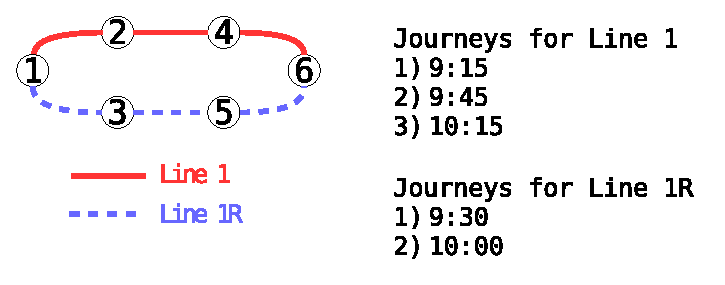
\includegraphics[width=\textwidth]{example_network.eps}
\caption{An example network for our model, with two lines and five stops}
\label{fig:example_network}
\end{figure}

Users can be attached to trips, but we don't care about them yet.

\section{Relevant queries}
\label{seq:rq}
We are interested in solving two kinds of queries:

\begin{enumerate}[A)]
    \item Aggregation of passengers
    \item Movement patterns
\end{enumerate}

\section{Proposed Structures}
As of today, we are not aware of any indexing structure that would allow to efficiently represent trajectories that could also support all the kinds of queries described in Section~\ref{seq:rq}. For this reason, we propose two data structures, \acumm~and~\ctr. The first is targeted for queries of type A, solving most aggregation queries in constant time, while the later can be used for queries of type B.

\subsection{Common Structures}
Both \acumm and \ctr need a network representation to be operated, which is represented in the following components:

\begin{itemize}
    \item $lineStop_i(j)$ is the $j$th stop of line $l_i$
    \item $stopLine_i(j)$ is the $j$th line that makes a stop at the stop $s_i$
    \item $avgTime_i(j)$ is the average time in seconds that it takes for a vehicle of line $l_i$ to reach its $j$th stop from the start of a journey
    \item $initialTime_i(k)$ is the starting time of the journey $j_k$ for line $l_i$
\end{itemize}

All of them stored explicitly except for $initialTime$, which is compressed with sampled ZSTD.

\begin{algorithm}[H]
\SetKwData{l}{$l$}\SetKwData{lz}{l$_z$}\SetKwData{s}{s}\SetKwData{sz}{s$_z$}\SetKwData{ta}{t$_a$}\SetKwData{tz}{t$_z$}\SetKwData{pattern}{pattern}\SetKwData{left}{left}\SetKwData{right}{right}\SetKwData{csa}{CSA}\SetKwData{wmj}{WMJ}\SetKwData{leftzero}{left$_0$}\SetKwData{rightzero}{right$_0$}\SetKwData{i}{i}\SetKwData{z}{z}\SetKwData{ja}{j$_a$}\SetKwData{jz}{j$_z$}\SetKwData{n}{n}\SetKwData{ap}{a'}\SetKwData{zp}{z'}\SetKwData{offset}{offset}
 \SetKwFunction{GetBounds}{GetBounds}\SetKwFunction{GetJCodes}{GetJCodes}\SetKwFunction{GetCount}{GetCount}\SetKwFunction{GetPsi}{$\Psi$}\SetKwFunction{GetRangeSpecial}{GetRange$^*$}\SetKwFunction{bsearch}{binary\_search}\SetKwFunction{lbound}{lower\_bound}\SetKwFunction{ubound}{upper\_bound}
 \SetKwProg{Fn}{Function}{\string:}{}
 
 \Fn{\GetJCodes{\l,\s,\ta,\tz}}{
 \KwData{line \l, stop \s, times \ta,\tz}
 \KwResult{jcodes for \ta and \tz}
 \BlankLine
 \offset $\leftarrow$ $avgTime_{\l}(\bsearch{$lineStop_\l$, \s})$\;
 \Return{\lbound{$initialTime_\l$, \ta-\offset}, \ubound{$initialTime_\l$, \tz-\offset}}\;
 }
 
 \caption{Obtaining the codes of the journeys from the line \l that should arrive to the stop \s within the time range given by \ta and \tz}
\end{algorithm}

\subsection{\acumm}
Tirso please explain what you did. Did you use bitmaps for partial sums? Matrices? Any other trick from inverted lists? Also explain how queries are solved again, in detail.

\subsection{\ctr}
A user trip can be represented by the stops from the transportation system boarded by a user, so from now on we will consider a trip as a sequence of triplets $<s,l,j>$, where $s$, $l$ are, respectively, stop and line identifiers, while $j$ are the journey codes corresponding to the journeys that compose the trip. Additionally, as we are interested in knowing where the trips end, we also represent the last stop where the user has alighted, which line and journey will logically match the line and journey of the last boarding stop. Although it is generally hard to obtain information about the last destination stop of a trip, many transportation companies are investing effort in providing it, either by implementing systems to keep track of users as they leave their system or estimating it based on previous trips made by that user\marginnote{[CITATION NEEDED]}.

We use three complementary structures to represent each component of the sequence:
\begin{enumerate}[(i)]
    \item CSA with special and circular $\$$
    \item lines WM "forest"
    \item jcodes WM
\end{enumerate}

\begin{figure}
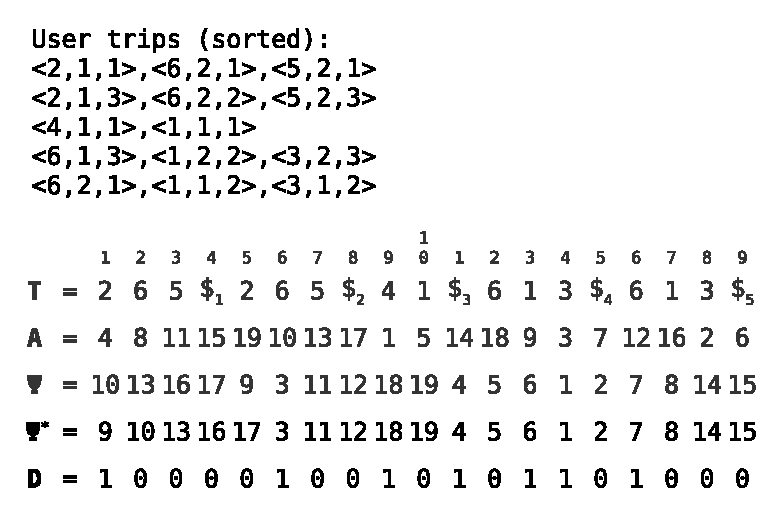
\includegraphics[width=\textwidth]{example_trips.eps}
\caption{An example of five trips represented on \ctr}
\label{fig:example_ctr}
\end{figure}

This construction allows us to answer from x to y with just (i).

Then we can use (ii) to restrict lines.

And finally we can restrict times by finding out the right jcodes and filtering through (iii).

Theoretically we can answer anything. It's a representation, after all...

\begin{algorithm}[H]
\SetKwData{la}{$l_a$}\SetKwData{lz}{$l_z$}\SetKwData{sa}{s$_a$}\SetKwData{sz}{s$_z$}\SetKwData{ta}{t$_a$}\SetKwData{tz}{t$_z$}\SetKwData{pattern}{pattern}\SetKwData{left}{left}\SetKwData{right}{right}\SetKwData{csa}{CSA}\SetKwData{wmj}{WMJ}\SetKwData{leftzero}{left$_0$}\SetKwData{rightzero}{right$_0$}\SetKwData{a}{a}\SetKwData{z}{z}\SetKwData{ja}{j$_a$}\SetKwData{jz}{j$_z$}\SetKwData{n}{n}\SetKwData{ap}{a'}\SetKwData{zp}{z'}\SetKwData{offset}{offset}
 \SetKwFunction{GetRange}{GetRange}\SetKwFunction{GetJCodes}{GetJCodes}\SetKwFunction{GetCount}{GetCount}\SetKwFunction{GetPsi}{$\Psi$}\SetKwFunction{GetRangeSpecial}{GetRange$^*$}\SetKwFunction{wml}{WML}\SetKwFunction{TrackUp}{TrackUp}\SetKwFunction{Select}{Select}\SetKwFunction{fxy}{FromXtoY\_full}
 \SetKwProg{Fn}{Function}{\string:}{}
 
 \Fn{\fxy{\la,\lz,\sa,\sz,\ta,\tz,\n}}{
 \KwData{lines \la,\lz, stops \sa,\sz, times \ta,\tz and length of the sequence \n}
 \KwResult{Number of occurences}
 \BlankLine
 \pattern $\leftarrow \{\sz,0,\sa\}$\;
 \left,\right $\leftarrow$ \GetRange{\csa, $0$, \n, \pattern}\;
 \leftzero $\leftarrow$ \GetPsi{\csa, \left}\;
 \rightzero $\leftarrow$ \GetPsi{\csa, \right}\;
 \tcp{\right-\left = \rightzero-\leftzero}
 \a,\z $\leftarrow$ \GetRange{\wml{$0$},\leftzero,\rightzero,\la}\;
 \ja,\jz $\leftarrow$ \GetJCodes{\la,\sa,\ta,\tz}\;
 \a,\z $\leftarrow$ \GetRangeSpecial{\wmj,\a,\z,\ja,\jz}\;
 \ap $\leftarrow$ \TrackUp{\wml{$0$},\a}\;
 \zp $\leftarrow$ \TrackUp{\wml{$0$},\z}\;
 \tcp{\z-\a = \zp-\ap}
 \offset $\leftarrow$ \Select{\csa,\sz}\;
 \a,\z $\leftarrow$ \GetRange{\wml{\sz},\left-\offset~$+$~\ap-\leftzero,
 \left-\offset~$+$~\ap-\leftzero,\lz}\;
 \ja,\jz $\leftarrow$ \GetJCodes{\lz,\sz,\ta,\tz}\;
 \Return{\GetCount{\wmj,\offset~+~\a,\offset~+~\z,\ja,\jz}}\;
 }
 
 \caption{Querying for all features on \ctr where \DataSty{CSA}, \DataSty{WML} and \DataSty{WMJ} are structures (i), (ii) and (iii), respectively}
\end{algorithm}


\section{Experiments}
For space, I propose to compare with our previous structures and with a plain representation using bits per symbol (bps). Otherwise, the baseline we select for our $\%$ can be misleading.

For time, we will compare against SPIRE 2018, and maybe, IF WE HAVE TIME, with a plain postgresql baseline. Experiments will be executed in Compostela2 or whatever we'll have available.

\section{Conclusions}
Speak about how cool would it be to have a single structure that could to it all. Pitch for our next paper with Gonzalo!

\subsection{A Subsection Sample}
Please note that the first paragraph of a section or subsection is
not indented. The first paragraph that follows a table, figure,
equation etc. does not need an indent, either.

Subsequent paragraphs, however, are indented.

\subsubsection{Sample Heading (Third Level)} Only two levels of
headings should be numbered. Lower level headings remain unnumbered;
they are formatted as run-in headings.

\paragraph{Sample Heading (Fourth Level)}
The contribution should contain no more than four levels of
headings. Table~\ref{tab1} gives a summary of all heading levels.

\begin{table}
\caption{Table captions should be placed above the
tables.}\label{tab1}
\begin{tabular}{|l|l|l|}
\hline
Heading level &  Example & Font size and style\\
\hline
Title (centered) &  {\Large\bfseries Lecture Notes} & 14 point, bold\\
1st-level heading &  {\large\bfseries 1 Introduction} & 12 point, bold\\
2nd-level heading & {\bfseries 2.1 Printing Area} & 10 point, bold\\
3rd-level heading & {\bfseries Run-in Heading in Bold.} Text follows & 10 point, bold\\
4th-level heading & {\itshape Lowest Level Heading.} Text follows & 10 point, italic\\
\hline
\end{tabular}
\end{table}


\noindent Displayed equations are centered and set on a separate
line.
\begin{equation}
x + y = z
\end{equation}
Please try to avoid rasterized images for line-art diagrams and
schemas. Whenever possible, use vector graphics instead (see
Fig.~\ref{fig1}).

\begin{figure}
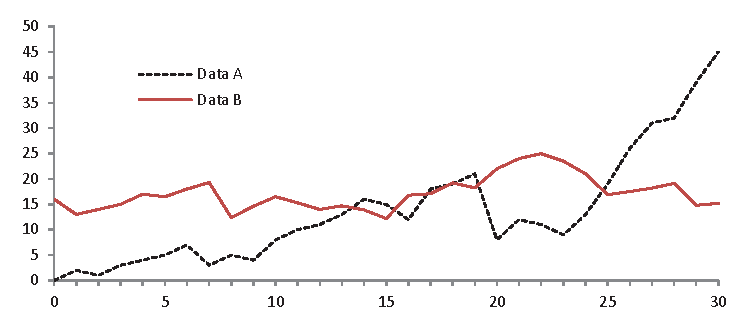
\includegraphics[width=\textwidth]{fig1.eps}
\caption{A figure caption is always placed below the illustration.
Please note that short captions are centered, while long ones are
justified by the macro package automatically.} \label{fig1}
\end{figure}

\begin{theorem}
This is a sample theorem. The run-in heading is set in bold, while
the following text appears in italics. Definitions, lemmas,
propositions, and corollaries are styled the same way.
\end{theorem}
%
% the environments 'definition', 'lemma', 'proposition', 'corollary',
% 'remark', and 'example' are defined in the LLNCS documentclass as well.
%
\begin{proof}
Proofs, examples, and remarks have the initial word in italics,
while the following text appears in normal font.
\end{proof}

%
% ---- Bibliography ----
%
% BibTeX users should specify bibliography style 'splncs04'.
% References will then be sorted and formatted in the correct style.

\bibliographystyle{splncs04}
\bibliography{refs}

\end{document}
